% IMPORTANT NOTE: This document was built out of another. This document here was the basis. Simplified and modified the document for this class.
% https://www.overleaf.com/latex/templates/capstone-project-template/fcqkgvbwynzz

\documentclass[12pt, a4paper,oneside]{book}
\newcommand{\re}{\mathrm{e}}
\newcommand{\ri}{\mathrm{i}}
\newcommand{\rd}{\mathrm{d}}
\def\semicolon{\nobreak\mskip2mu\mathpunct{}\nonscript\mkern-\thinmuskip{;}
\mskip6muplus1mu\relax} % This defines the semicolon command

        % allows index generation
\usepackage{graphicx}        % standard LaTeX graphics tool
                             % when including figure files
\usepackage{multicol}        % used for the two-column index




\usepackage{color,tikz}


\usepackage{amsmath,eucal,amssymb}
\usepackage{mathrsfs,graphicx,texdraw}
\usepackage{fancyhdr,framed}
\usepackage{tikz, tikz-3dplot}
\usepackage{tkz-euclide}
\usetikzlibrary{decorations.fractals}
\usetikzlibrary{decorations.footprints}

\usepackage{palatino}

\usepackage[latin1]{inputenc}

\usepackage[T1]{fontenc}

% These are LMU's two colors. Feel free to change out where some blue is present for crimson if you think it looks better
\definecolor{mycrimson}{HTML}{AB0C2F} %%% LMU CRIMSON
\definecolor{myblue}{HTML}{0076A5} %%% LMU BLUE


\def\grole{\mathrel{\mathchoice {\vcenter{\offinterlineskip\halign{\hfil
$\displaystyle##$\hfil\cr>\cr\noalign{\vskip-1.5pt}<\cr}}}
{\vcenter{\offinterlineskip\halign{\hfil$\textstyle##$\hfil\cr
>\cr\noalign{\vskip-1.5pt}<\cr}}}
{\vcenter{\offinterlineskip\halign{\hfil$\scriptstyle##$\hfil\cr
>\cr\noalign{\vskip-1pt}<\cr}}}
{\vcenter{\offinterlineskip\halign{\hfil$\scriptscriptstyle##$\hfil\cr
>\cr\noalign{\vskip-0.5pt}<\cr}}}}}

\newenvironment{rcases}
  {\left.\begin{aligned}}
  {\end{aligned}\right\rbrace}

\newenvironment{lcases}
  {\left\lbrace\begin{aligned}}
  {\end{aligned}\right.}

\newtheorem{theorem}{Theorem}[section]
\newtheorem{lemma}[theorem]{Lemma}
\newtheorem{proposition}[theorem]{Proposition}
\newtheorem{corollary}[theorem]{Corollary}
\newtheorem{definition}[theorem]{Definition}
\newtheorem{example}[theorem]{Example}
\newtheorem{remark}[theorem]{Remark}

\newenvironment{proof}[1][Proof]{\begin{trivlist}
\item[\hskip \labelsep {\bfseries #1}]}{\end{trivlist}}
\newenvironment{solution}[1][Solution]{\begin{trivlist}
\item[\hskip \labelsep {\bfseries #1}]}{\end{trivlist}}

\newcommand{\qed}{\nobreak \ifvmode \relax \else
      \ifdim\lastskip<1.5em \hskip-\lastskip
      \hskip1.5em plus0em minus0.5em \fi \nobreak
      \vrule height0.75em width0.5em depth0.25em\fi}

\numberwithin{equation}{section}
\def\Ad{{\mbox{Ad}}}
\def\im{{\mbox{Im}}}
\def\Re{{\mbox{Re}\;}}
\def\ad{\mathrm{ad\,}}
\def\openone{\leavevmode\hbox{\small1\kern-3.3pt\normalsize1}}
\def\Res{\mathop{\mbox{Res}\,}\limits}
\def\biglb{\big[\hspace*{-.7mm}\big[}
\def\bigrb{\big]\hspace*{-.7mm}\big]}


\def\bigrbt{\mathop{\bigrb }\limits_{\widetilde{\;}}}
\def\biggrbt{\mathop{\biggrb }\limits_{\widetilde{\;}}}
\def\Bigrbt{\mathop{\Bigrb }\limits_{\widetilde{\;}}}
\def\Biggrbt{\mathop{\Biggrb }\limits_{\widetilde{\;}}}

\def\bPhi{\mathbf{\Phi}}
\def\bM{\mathbf{M}}
\def\bm{\mathbf{m}}
\def\bbbc{{\Bbb C}}
\def\bbbr{{\Bbb R}}
\def\bbbz{{\Bbb Z}}
\def\bbbs{{\Bbb S}}
\def\diag{\mbox{diag}\,}
\def\tr{\mbox{tr}\,}

\textwidth=17cm   \textheight=24.5cm \voffset=-2cm

\evensidemargin=-0.5cm \oddsidemargin=-0.5cm

 \renewcommand{\baselinestretch}{1.5}

%%%%%%%%fancy header%%%%%%%%%%%%%%%%%

\usepackage{fancyhdr}
\pagestyle{fancy}
\usepackage{calc}
\newlength{\pageoffset}
\setlength{\pageoffset}{0cm}% use whatever you like
\fancyheadoffset[LE,RO]{\pageoffset}
\renewcommand{\chaptermark}[1]{\markboth{#1}{}}
\renewcommand{\sectionmark}[1]{\markright{\thesection\ #1}}
\fancyhf{}
\fancyhead[LE]{\makebox[\pageoffset][l]{\thepage}\hfill\leftmark}
\fancyhead[RO]{\rightmark\hfill\makebox[\pageoffset][r]{\thepage}}
\fancypagestyle{plain}{%
    \fancyhead{} % get rid of headers
    \renewcommand{\headrulewidth}{0pt} % and the line
}

%%%%%%%%%%%%%%%%%%%%%%%%%%%%%%%%%%%%

\arraycolsep=2pt

%%%%Fancy Chapter%%%

%\usepackage{lmodern}
\usepackage{graphicx}
\usepackage{xcolor}
\usepackage{titlesec}
\usepackage{microtype}
\usepackage{lipsum}

%\definecolor{myblue}{RGB}{0,82,155}

\titleformat{\chapter}[display]
  {\normalfont\bfseries\color{myblue}}
  {\filleft\hspace*{-60pt}%
    \rotatebox[origin=c]{90}{%
      \normalfont\color{black}\Large%
        \textls[180]{\textsc{\chaptertitlename}}%
    }\hspace{10pt}%
    {\setlength\fboxsep{0pt}%
    \colorbox{myblue}{\parbox[c][3cm][c]{2.5cm}{%
      \centering\color{white}\fontsize{80}{90}\selectfont\thechapter}%
    }}%
  }
  {10pt}
  {\titlerule[2.5pt]\vskip3pt\titlerule\vskip4pt\LARGE\sffamily}

% hyperref should be loaded after all other packages
% aliascnt is needed to get \autoref (from hyperref) to work correctly with custom amsthm theorems
\usepackage{aliascnt}
\usepackage[colorlinks,linkcolor=myblue,citecolor=mygreen]{hyperref}


%%% Make Necessry Changes Here Only %%% 

\newcommand{\MyName}{Ryan Ramsdell} %% Change this to your name %%
\newcommand{\MyLink}{\url{github.com/Un3qual/schoolscript_backend}} %% Change this to your link %%

\newcommand{\ProjectTitle}{School Script} %% Change this to your project title %%
\newcommand{\SuperviserName}{Insert Supervisor's name }  %% Change this to your project supervisor. If you do not have a supervisor, comment out the line indicated below  %%

%%%%%%%%%%%%%%%%%%%%%%%%%%

%%% Not necessary to change anything below this line, excluding supervisor. However, if you want the spacing on the title page changed, feel free to mess with the margins. %%%
\begin{document}
\thispagestyle{empty}

\begin{center}
{\LARGE \bf \sl Loyola Marymount University}

{\LARGE \bf Department of Computer Science}

\noindent\textcolor{mycrimson}{\rule{\linewidth}{4.8pt}}

\vspace{2.5cm}
{\LARGE{\color{myblue}  \ProjectTitle{}}}

\vspace{1.5cm}

{\Large \bf \MyName{}}

\vspace{11cm} % If you have a logo and would like to insert it, you can insert it here and change the "vspace" to adjust. 


{\color{myblue} \bf \MyLink{}}

\vspace{2cm}

% {\Large {Supervisor:} {\color{myblue} \bf  \SuperviserName{}}} % COMMENT OUT/DELETE THIS LINE IF YOU DO NOT HAVE A SUPERVISOR

\vspace{.25cm}
\noindent\textcolor{mycrimson}{\rule{\linewidth}{4.8pt}}
\vspace{1cm}
{\Large \today }\\[4pt] % Will always display today's date (UTC)


\end{center}

% END OF TITLE PAGE!

\newpage

\tableofcontents
% \listoffigures
% \listoftables

%%% Do not change anything  above %%%

\chapter{Introduction}\label{ch:1}

If you would like to include a project introduction, include it here! If not, feel free to delete this chapter and text (Note: you will need to adjust the following chapter labels)


\chapter{Project Pitch}\label{ch:2}

{\large Problem Statement}\\
Main issue: It's very difficult to transfer prescriptions between a pharmacy close to your college and one near your home when you go home for breaks\\
Side issues: Mental, covid, and sexual health services are often taboo and difficult to find on college campuses
\\\\{\large Proposed Solution}\\
Main solution: Ship prescriptions to college, all in one box, and ship home when summer starts. Usable through a website and an app. Will use TruePill as a private label pharmacy and fulfillment provider.\\
Side solution: Offer telehealth for mental health for students, included in their tuition, sell test kits in student stores and other places on campus
\\\\{\large Target Audience}\\
College Students
\\\\{\large Project Scope}\\
End of semester: Website and/or app that calls a stubbed API allowing users to manage fake prescriptions\\
Stretch goal: Interact with TruePill API and actually fill prescriptions


\chapter{Project Timeline}

Project timeline here!

\section{Initial Planned Timeline}

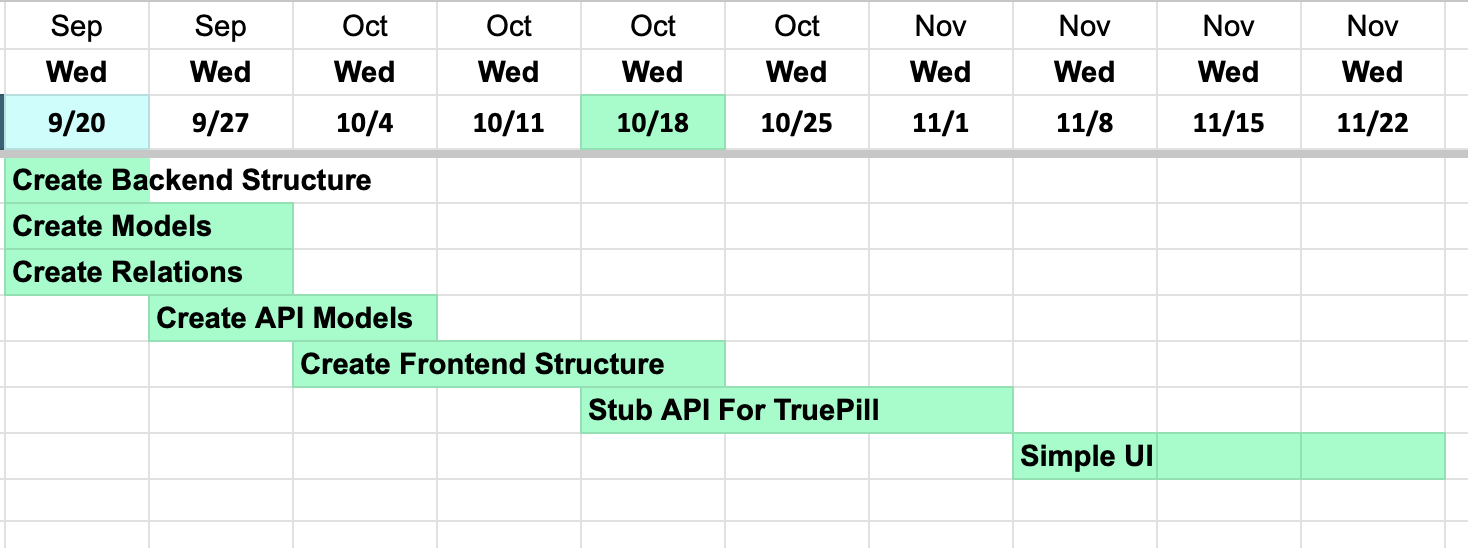
\includegraphics[scale=0.7]{orig_timeline.png} % inside [] you can scale, or set width/height


\section{Final project schedule status}\label{sec:3.2}
I am on schedule, however I have decided to do a standard, server rendered UI,
rather than a GraphQL API and a seperate React frontend.
% \includegraphics[width=15cm, height=10cm]{timeline.png} % setting width and height does not maintain original dimensions


\chapter{Testing}
I test the project by simply using it in the intended manner, with fake accounts.

\chapter{Project Installation Guide}
Elixir and Docker must be installed. Docker can be installed from their website. For elixir, I like to use the {\em asdf} version manager.
Once installed (I used {\em homebrew}), run:
\begin{center}
  \texttt{asdf install elixir 1.15.6}\\
  \texttt{asdf install erlang 26.1.2}\\
  \texttt{asdf global elixir 1.15.6}\\
  \texttt{asdf global erlang 26.1.2}
\end{center}
To start the database and web server, simply open two terminal tabs. In one, enter \texttt{docker compose up}.
In the other, run \texttt{iex -S mix phx.server} to start the development web server.
Visit \texttt{localhost:4000} in your web browser. 

\chapter{Passing the Baton}
This is a project that I intend to continue with on my own in the future, 
so there is not much to do in the way of passing the baton to someone else,
however, there are better practices I could be using that would make this project 
easier to work on as a team, such as better documentation and adding unit tests.







\end{document}

